\begin{figure}
    \centering
    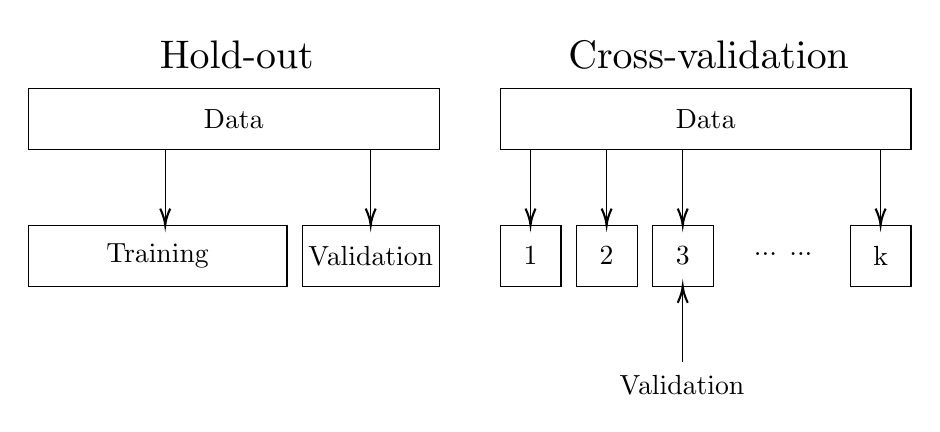
\begin{tikzpicture}[x=0.55pt,y=0.55pt,yscale=-1,xscale=1]
        %Shape: Rectangle [id:dp30782299997247864] 
        \draw   (30,40) -- (300,40) -- (300,80) -- (30,80) -- cycle ;
        %Shape: Rectangle [id:dp5159914550919137] 
        \draw   (340,40) -- (610,40) -- (610,80) -- (340,80) -- cycle ;
        %Shape: Rectangle [id:dp8069194161926109] 
        \draw   (30,130) -- (200,130) -- (200,170) -- (30,170) -- cycle ;
        %Shape: Rectangle [id:dp959684597440048] 
        \draw   (210,130) -- (300,130) -- (300,170) -- (210,170) -- cycle ;
        %Shape: Rectangle [id:dp8001671544362841] 
        \draw   (340,130) -- (380,130) -- (380,170) -- (340,170) -- cycle ;
        %Shape: Rectangle [id:dp19700561762726387] 
        \draw   (570,130) -- (610,130) -- (610,170) -- (570,170) -- cycle ;
        %Shape: Rectangle [id:dp6964850406597634] 
        \draw   (390,130) -- (430,130) -- (430,170) -- (390,170) -- cycle ;
        %Shape: Rectangle [id:dp5278376415103712] 
        \draw   (440,130) -- (480,130) -- (480,170) -- (440,170) -- cycle ;
        %Straight Lines [id:da17033992216894744] 
        \draw    (360,80) -- (360,128) ;
        \draw [shift={(360,130)}, rotate = 270] [color={rgb, 255:red, 0; green, 0; blue, 0 }  ][line width=0.75]    (10.93,-3.29) .. controls (6.95,-1.4) and (3.31,-0.3) .. (0,0) .. controls (3.31,0.3) and (6.95,1.4) .. (10.93,3.29)   ;
        
        %Straight Lines [id:da5076595148790187] 
        \draw    (410,80) -- (410,128) ;
        \draw [shift={(410,130)}, rotate = 270] [color={rgb, 255:red, 0; green, 0; blue, 0 }  ][line width=0.75]    (10.93,-3.29) .. controls (6.95,-1.4) and (3.31,-0.3) .. (0,0) .. controls (3.31,0.3) and (6.95,1.4) .. (10.93,3.29)   ;
        
        %Straight Lines [id:da6592490936454037] 
        \draw    (460,80) -- (460,128) ;
        \draw [shift={(460,130)}, rotate = 270] [color={rgb, 255:red, 0; green, 0; blue, 0 }  ][line width=0.75]    (10.93,-3.29) .. controls (6.95,-1.4) and (3.31,-0.3) .. (0,0) .. controls (3.31,0.3) and (6.95,1.4) .. (10.93,3.29)   ;
        
        %Straight Lines [id:da8377856383779624] 
        \draw    (590,80) -- (590,128) ;
        \draw [shift={(590,130)}, rotate = 270] [color={rgb, 255:red, 0; green, 0; blue, 0 }  ][line width=0.75]    (10.93,-3.29) .. controls (6.95,-1.4) and (3.31,-0.3) .. (0,0) .. controls (3.31,0.3) and (6.95,1.4) .. (10.93,3.29)   ;
        
        %Straight Lines [id:da5318453015444125] 
        \draw    (120,80) -- (120,128) ;
        \draw [shift={(120,130)}, rotate = 270] [color={rgb, 255:red, 0; green, 0; blue, 0 }  ][line width=0.75]    (10.93,-3.29) .. controls (6.95,-1.4) and (3.31,-0.3) .. (0,0) .. controls (3.31,0.3) and (6.95,1.4) .. (10.93,3.29)   ;
        
        %Straight Lines [id:da5175740274992974] 
        \draw    (255,80) -- (255,128) ;
        \draw [shift={(255,130)}, rotate = 270] [color={rgb, 255:red, 0; green, 0; blue, 0 }  ][line width=0.75]    (10.93,-3.29) .. controls (6.95,-1.4) and (3.31,-0.3) .. (0,0) .. controls (3.31,0.3) and (6.95,1.4) .. (10.93,3.29)   ;
        
        %Straight Lines [id:da7508158168507306] 
        \draw    (460,172) -- (460,220) ;
        
        \draw [shift={(460,170)}, rotate = 90] [color={rgb, 255:red, 0; green, 0; blue, 0 }  ][line width=0.75]    (10.93,-3.29) .. controls (6.95,-1.4) and (3.31,-0.3) .. (0,0) .. controls (3.31,0.3) and (6.95,1.4) .. (10.93,3.29)   ;
        
        % Text Node
        \draw (255,150) node  [align=left] {Validation};
        % Text Node
        \draw (165,60) node  [align=left] {Data};
        % Text Node
        \draw (475,60) node  [align=left] {Data};
        % Text Node
        \draw (115,150) node  [align=left] {Training};
        % Text Node
        \draw (360,150) node  [align=left] {1};
        % Text Node
        \draw (410,150) node  [align=left] {2};
        % Text Node
        \draw (460,150) node  [align=left] {3};
        % Text Node
        \draw (590,150) node  [align=left] {k};
        % Text Node
        \draw (526,149) node  [align=left] {... ...};
        % Text Node
        \draw (167,18) node [scale=1.44] [align=left] {Hold-out};
        % Text Node
        \draw (477,18) node [scale=1.44] [align=left] {Cross-validation};
        % Text Node
        \draw (459.5,235) node  [align=left] {Validation};
    \end{tikzpicture}
    \caption{Difference between validating using an hold-out sample and \(k\)-fold cross-validation. While in the first case part of data are is hold out, in the second one a re-sampling technique is used.}
    \label{holdout_vs_crossvalidation}
\end{figure}